% TCC de Física experimental (classe abntex2)
% Modelo do ÉguaTex (https://www.eguatex.com.br), em domínio público pela licença CC0 1.0:
% use, modifique e distribua sem pedir permissão e sem citar a origem.
%
% Compile com pdfLaTeX e BibTeX (o ÉguaTex faz isso sozinho).
% Arquivos:
%   main.tex            preâmbulo, elementos pré-textuais e pós-textuais
%   capitulos/*.tex     um arquivo por capítulo, na ordem dos \input abaixo
%   dados.dat           medidas usadas na tabela, no gráfico e no ajuste
%   referencias.bib     bibliografia no formato BibTeX

\documentclass[
  12pt,            % corpo 12 para o texto, como pede a NBR 14724
  oneside,         % troque por twoside para imprimir frente e verso
  a4paper,
  english,         % idioma do abstract
  brazilian,       % idioma principal (o último da lista)
]{abntex2}

% ---------- idioma, fontes e microtipografia ----------
\usepackage[T1]{fontenc}
\usepackage[utf8]{inputenc}
\usepackage{lmodern}
\usepackage{microtype}

% ---------- matemática, unidades, tabelas e figuras ----------
\usepackage{amsmath}
\usepackage{siunitx}
\sisetup{locale=FR, output-decimal-marker={,}, separate-uncertainty=true, per-mode=symbol}
\usepackage{booktabs}
\usepackage{xcolor}
\usepackage{tikz}
\usetikzlibrary{arrows.meta, patterns, decorations.pathmorphing, calc, babel}
\usepackage{pgfplots}
\usepackage{pgfplotstable}
\pgfplotsset{compat=1.18}

% ---------- referências no padrão ABNT ----------
% A classe abntex2 já carrega o hyperref; aqui só ajustamos as opções.
\hypersetup{hidelinks}
\usepackage[alf]{abntex2cite}

% ---------- instruções de preenchimento ----------
% Os textos em cinza explicam o que escrever em cada parte.
% Troque \instrucoestrue por \instrucoesfalse para esconder todos de uma vez.
\newif\ifinstrucoes
\instrucoestrue
\newcommand{\instrucao}[1]{\ifinstrucoes{\color{gray}\small\itshape #1\par}\fi}

% ---------- dados do trabalho: preencha aqui ----------
\titulo{Medida da velocidade do som no ar com um tubo de ressonância}
\autor{Nome do autor}
\local{Cidade}
\data{Ano}
\orientador{Prof. Dr. Nome do orientador}
\coorientador{Prof.\textsuperscript{a} Dr.\textsuperscript{a} Nome da coorientadora}
\instituicao{%
  Universidade Federal Exemplo\par
  Instituto de Ciências Exatas e Naturais\par
  Faculdade de Física}
\tipotrabalho{Trabalho de Conclusão de Curso}
\preambulo{Trabalho de Conclusão de Curso apresentado à Faculdade de Física da Universidade Federal Exemplo como requisito parcial para a obtenção do grau de Bacharel em Física.}

\makeatletter
\hypersetup{pdftitle={\@title}, pdfauthor={\@author}, pdfsubject={\imprimirpreambulo}}
\makeatother

% ---------- cálculos a partir das medidas (arquivo dados.dat) ----------
% O ajuste linear ponderado de L em função de x = (2n-1)/4 dá o comprimento de onda
% (coeficiente angular) e a correção de extremidade (coeficiente linear com sinal trocado).
\pgfplotstableread{dados.dat}\medidas
\pgfplotstablecreatecol[linear regression={x=x, y=L, variance=sL}]{ajuste}\medidas
\pgfmathsetmacro{\lambdaAjuste}{\pgfplotstableregressiona}
\pgfmathsetmacro{\correcao}{-1*\pgfplotstableregressionb}
% Frequência do gerador (Hz) e incerteza do coeficiente angular (m), calculada com as
% equações do Apêndice A. Troque pelos seus valores.
\newcommand{\frequencia}{1000}
\newcommand{\incertezaLambda}{0.00096}
\pgfmathsetmacro{\velocidade}{\frequencia*\lambdaAjuste}
\pgfmathsetmacro{\incertezaVelocidade}{\frequencia*\incertezaLambda}

\begin{document}

% ======================================================================
% Elementos pré-textuais
% ======================================================================
\pretextual

\imprimircapa
% As chaves vazias depois de \imprimirfolhaderosto evitam um erro conhecido da classe.
\imprimirfolhaderosto{}

\begin{folhadeaprovacao}
  \begin{center}
    {\ABNTEXchapterfont\large\imprimirautor}

    \vspace*{\fill}\vspace*{\fill}
    {\ABNTEXchapterfont\bfseries\Large\imprimirtitulo}
    \vspace*{\fill}

    \hspace{.45\textwidth}
    \begin{minipage}{.5\textwidth}
      \imprimirpreambulo
    \end{minipage}%
    \vspace*{\fill}
  \end{center}

  Trabalho aprovado. \imprimirlocal, dia de mês de \imprimirdata.

  \assinatura{\textbf{\imprimirorientador} \\ Orientador}
  \assinatura{\textbf{Prof. Dr. Nome do membro da banca} \\ Universidade Federal Exemplo}
  \assinatura{\textbf{Prof.\textsuperscript{a} Dr.\textsuperscript{a} Nome da membro da banca} \\ Instituição}

  \begin{center}
    \vspace*{0.5cm}
    {\large\imprimirlocal}
    \par
    {\large\imprimirdata}
    \vspace*{1cm}
  \end{center}
\end{folhadeaprovacao}

\begin{agradecimentos}
  \instrucao{Opcional. Em poucas linhas, agradeça a quem contribuiu de fato: orientação, técnicos do laboratório, agência de fomento (com o número do processo).}
  Agradeço ao orientador, à equipe técnica do Laboratório de Física e aos colegas que ajudaram na montagem experimental.
\end{agradecimentos}

\begin{resumo}
  \instrucao{Um parágrafo de 150 a 500 palavras (NBR 6028): objetivo, método, resultado principal com incerteza e conclusão. Escreva por último.}
  Este trabalho determina a velocidade do som no ar a partir das ressonâncias de uma coluna de ar em um tubo fechado em uma das extremidades. Para uma frequência fixa de \qty{\frequencia}{\hertz}, foram medidas as seis primeiras posições de ressonância, e a relação linear entre a posição e a ordem da ressonância foi ajustada pelo método dos mínimos quadrados ponderados. O coeficiente angular fornece o comprimento de onda e, com ele, $v = \qty[round-mode=uncertainty]{\velocidade \pm \incertezaVelocidade}{\metre\per\second}$, compatível com o valor previsto para a temperatura do laboratório. O coeficiente linear dá a correção de extremidade do tubo, comparada com a estimativa teórica.

  \textbf{Palavras-chave}: velocidade do som. Tubo de ressonância. Ondas estacionárias. Incerteza de medição.
\end{resumo}

\begin{resumo}[Abstract]
  \begin{otherlanguage*}{english}
    \instrucao{Tradução fiel do resumo para o inglês, com as mesmas informações.}
    This work determines the speed of sound in air from the resonances of an air column in a tube closed at one end. For a fixed frequency, the first six resonance positions were measured and fitted by weighted least squares. The slope gives the wavelength and the speed of sound, which agrees with the value expected at the laboratory temperature.

    \vspace{\onelineskip}
    \noindent\textbf{Keywords}: speed of sound. Resonance tube. Standing waves. Measurement uncertainty.
  \end{otherlanguage*}
\end{resumo}

\pdfbookmark[0]{\listfigurename}{lof}
\listoffigures*
\cleardoublepage

\pdfbookmark[0]{\listtablename}{lot}
\listoftables*
\cleardoublepage

\begin{siglas}
  \item[GUM] Guia para a Expressão da Incerteza de Medição
  \item[SI] Sistema Internacional de Unidades
\end{siglas}

\begin{simbolos}
  \item[$f$] Frequência do gerador de sinais
  \item[$\lambda$] Comprimento de onda
  \item[$L_n$] Posição da $n$-ésima ressonância
  \item[$e$] Correção de extremidade do tubo
  \item[$v$] Velocidade do som no ar
\end{simbolos}

\pdfbookmark[0]{\contentsname}{toc}
\tableofcontents*
\cleardoublepage

% ======================================================================
% Elementos textuais: um arquivo por capítulo
% ======================================================================
\textual

% ======================================================================
\chapter{Introdução}
\label{cap:introducao}
% ======================================================================
\instrucao{De duas a quatro páginas. Apresente o fenômeno, por que medir a grandeza escolhida e o que já se sabe sobre ela. Termine com o objetivo geral, os objetivos específicos e a organização do texto.}

A velocidade do som em um gás depende da temperatura e da composição do meio, e sua medida é um dos experimentos clássicos de ondas mecânicas \cite{halliday2016}. Em um tubo fechado em uma extremidade, as ondas sonoras formam ondas estacionárias apenas para comprimentos de coluna bem definidos, o que permite obter o comprimento de onda com uma trena e um gerador de frequência \cite{nussenzveig2014}.

\section{Objetivos}

O objetivo geral deste trabalho é determinar a velocidade do som no ar, com a incerteza expressa segundo o GUM \cite{jcgm2008}. Os objetivos específicos são:
\begin{alineas}
  \item montar um tubo de ressonância com coluna de ar ajustável;
  \item medir as posições de ressonância para uma frequência fixa;
  \item ajustar a relação linear entre a posição e a ordem da ressonância;
  \item comparar o resultado com o valor previsto para a temperatura ambiente.
\end{alineas}

\section{Organização do trabalho}

O \autoref{cap:fundamentacao} apresenta o modelo de ondas estacionárias em tubos. O \autoref{cap:metodologia} descreve a montagem e o procedimento. O \autoref{cap:resultados} traz as medidas, o ajuste e a discussão, e o \autoref{cap:conclusao} resume os resultados.

% ======================================================================
\chapter{Fundamentação teórica}
\label{cap:fundamentacao}
% ======================================================================
\instrucao{Apresente só a teoria que será usada na análise. Numere as equações, defina cada símbolo logo depois e cite a fonte. Cinco a dez páginas costumam bastar em um TCC experimental.}

\section{Ondas estacionárias em um tubo fechado}

Em um tubo fechado em uma extremidade e aberto na outra, a extremidade fechada é um nó de deslocamento e a aberta é, aproximadamente, um ventre. As ressonâncias ocorrem quando o comprimento efetivo da coluna é um múltiplo ímpar de um quarto do comprimento de onda \cite{halliday2016}:
\begin{equation}
  L_n + e = (2n-1)\,\frac{\lambda}{4}, \qquad n = 1, 2, 3, \dots
  \label{eq:ressonancia}
\end{equation}
em que $L_n$ é a posição da $n$-ésima ressonância, medida a partir da boca do tubo, e $e$ é a correção de extremidade, que leva em conta o fato de o ventre se formar um pouco fora do tubo. Para um tubo de raio $r$, a estimativa usual é $e \approx 0{,}6\,r$.

Definindo $x_n = (2n-1)/4$, a Equação~\eqref{eq:ressonancia} vira uma reta:
\begin{equation}
  L_n = \lambda\,x_n - e,
  \label{eq:reta}
\end{equation}
cujo coeficiente angular é o comprimento de onda. Com a frequência $f$ do gerador, a velocidade do som é
\begin{equation}
  v = f\,\lambda.
  \label{eq:velocidade}
\end{equation}

\section{Dependência com a temperatura}

Para um gás ideal, a velocidade do som cresce com a raiz quadrada da temperatura absoluta \cite{nussenzveig2014}. Para o ar seco, uma aproximação útil é
\begin{equation}
  v(T) = \qty{331.3}{\metre\per\second}\,\sqrt{1 + \frac{T}{\qty{273.15}{\celsius}}},
  \label{eq:temperatura}
\end{equation}
com $T$ em graus Celsius. A \qty{20}{\celsius}, ela dá cerca de \qty{343}{\metre\per\second}.

\section{Incerteza de medição}

A incerteza da velocidade vem da incerteza do comprimento de onda, já que a frequência do gerador é conhecida com incerteza relativa muito menor. Pela propagação de incertezas \cite{vuolo1996,taylor1997},
\begin{equation}
  \sigma_v = v\,\sqrt{\left(\frac{\sigma_\lambda}{\lambda}\right)^{2} + \left(\frac{\sigma_f}{f}\right)^{2}} \approx f\,\sigma_\lambda .
  \label{eq:incerteza}
\end{equation}

% ======================================================================
\chapter{Materiais e métodos}
\label{cap:metodologia}
% ======================================================================
\instrucao{Descreva a montagem com um desenho, liste os instrumentos com a resolução de cada um e conte o procedimento no passado, com detalhe suficiente para outra pessoa repetir o experimento.}

\section{Montagem experimental}

A \autoref{fig:montagem} mostra a montagem. Um tubo de acrílico de \qty{1.0}{\metre} contém água, cujo nível é controlado por um reservatório móvel ligado ao fundo do tubo. Um alto-falante, alimentado por um gerador de sinais, fica logo acima da boca do tubo.

\begin{figure}[htb]
  \caption{Esquema do tubo de ressonância com o nível da água ajustável.}
  \label{fig:montagem}
  \centering
  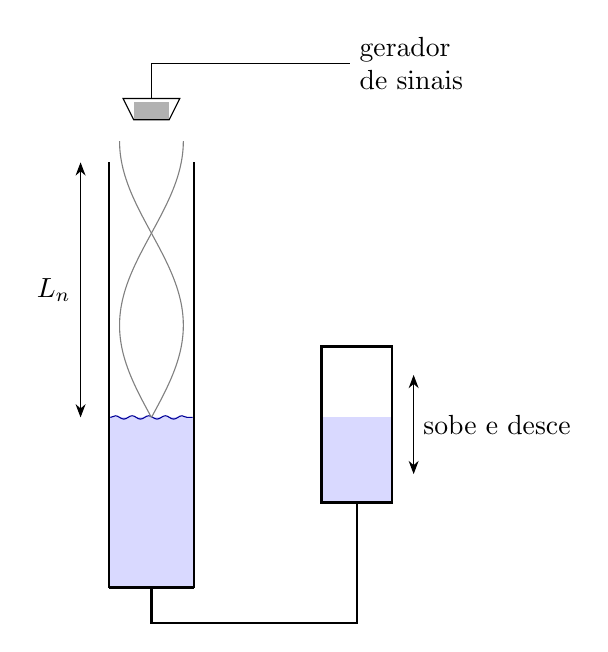
\begin{tikzpicture}[>=Stealth, scale=0.9]
    % tubo
    \draw[thick] (0,0) -- (0,6) (1.2,0) -- (1.2,6);
    \draw[thick] (0,0) -- (1.2,0);
    % água
    \fill[blue!15] (0.02,0.02) rectangle (1.18,2.4);
    \draw[blue!60!black, decorate, decoration={snake, amplitude=0.6pt, segment length=6pt}]
      (0.02,2.4) -- (1.18,2.4);
    % envoltória da onda estacionária na coluna de ar
    \draw[gray, domain=2.4:6.3, samples=60, smooth]
      plot ({0.6 + 0.45*sin(deg((\x-2.4)*pi/2.6))}, \x);
    \draw[gray, domain=2.4:6.3, samples=60, smooth]
      plot ({0.6 - 0.45*sin(deg((\x-2.4)*pi/2.6))}, \x);
    % alto-falante
    \fill[gray!60] (0.35,6.6) rectangle (0.85,6.85);
    \draw (0.2,6.9) -- (0.35,6.6) -- (0.85,6.6) -- (1.0,6.9) -- cycle;
    \draw (0.6,6.9) -- (0.6,7.4) -- (3.4,7.4) node[right, align=left] {gerador\\de sinais};
    % reservatório
    \draw[thick] (3,1.2) rectangle (4,3.4);
    \fill[blue!15] (3.02,1.22) rectangle (3.98,2.4);
    \draw[thick] (0.6,0) -- (0.6,-0.5) -- (3.5,-0.5) -- (3.5,1.2);
    \draw[<->] (4.3,1.6) -- (4.3,3.0) node[midway, right] {sobe e desce};
    % cota L
    \draw[<->] (-0.4,6) -- (-0.4,2.4) node[midway, left] {$L_n$};
  \end{tikzpicture}

  \legend{Fonte: elaborada pelo autor.}
\end{figure}

\section{Materiais}

\begin{alineas}
  \item tubo de acrílico com diâmetro interno de \qty{38}{\milli\metre};
  \item gerador de sinais senoidais com resolução de \qty{1}{\hertz};
  \item alto-falante de \qty{8}{\ohm};
  \item trena com resolução de \qty{1}{\milli\metre};
  \item termômetro com resolução de \qty{0.5}{\celsius}.
\end{alineas}

\section{Procedimento}

Com o gerador em \qty{\frequencia}{\hertz}, o nível da água foi abaixado lentamente a partir da boca do tubo. Cada ressonância foi identificada pelo máximo de intensidade sonora, e a posição do nível foi lida na trena. Cada posição foi medida cinco vezes, com aproximação por cima e por baixo, e a média foi adotada como $L_n$. A temperatura do ar foi registrada no início e no fim da série.

% ======================================================================
\chapter{Resultados e discussão}
\label{cap:resultados}
% ======================================================================
\instrucao{Mostre os dados em tabela com unidades e incertezas, o gráfico com barras de erro e o ajuste. Compare com a teoria ou com um valor de referência e discuta as fontes de incerteza mais importantes.}

\section{Posições de ressonância}

A \autoref{tab:dados} reúne as posições médias de ressonância e suas incertezas. A tabela é lida diretamente do arquivo \texttt{dados.dat}, o mesmo usado no gráfico.

\begin{table}[htb]
  \caption{Posições de ressonância para $f = \qty{\frequencia}{\hertz}$ (dados de exemplo).}
  \label{tab:dados}
  \centering
  \pgfplotstabletypeset[
    columns={n,x,L,sL},
    every head row/.style={before row=\toprule, after row=\midrule},
    every last row/.style={after row=\bottomrule},
    columns/n/.style={column name={$n$}},
    columns/x/.style={column name={$x_n = (2n-1)/4$}, fixed, fixed zerofill, precision=2, use comma},
    columns/L/.style={column name={$L_n$ (\unit{\metre})}, fixed, fixed zerofill, precision=3, use comma},
    columns/sL/.style={column name={$\sigma_L$ (\unit{\metre})}, fixed, fixed zerofill, precision=3, use comma},
  ]\medidas

  \legend{Fonte: elaborada pelo autor.}
\end{table}

\section{Ajuste linear}

A \autoref{fig:ajuste} mostra $L_n$ em função de $x_n$ com as barras de incerteza e a reta ajustada pela Equação~\eqref{eq:reta}. O coeficiente angular dá $\lambda = \qty[round-mode=uncertainty]{\lambdaAjuste \pm \incertezaLambda}{\metre}$, e o coeficiente linear dá a correção de extremidade $e = \qty[round-mode=places, round-precision=3]{\correcao}{\metre}$.

\begin{figure}[htb]
  \caption{Posição de ressonância em função de $x_n$, com a reta ajustada.}
  \label{fig:ajuste}
  \centering
  \begin{tikzpicture}
    \begin{axis}[
      width=0.8\linewidth, height=0.55\linewidth,
      xlabel={$x_n = (2n-1)/4$}, ylabel={$L_n$ (\unit{\metre})},
      xmin=0, xmax=3, ymin=0, ymax=1,
      grid=major, grid style={gray!25},
      legend pos=north west, legend cell align=left,
      /pgf/number format/use comma,
    ]
      \addplot[only marks, mark=square*, mark size=1.5pt,
        error bars/.cd, y dir=both, y explicit]
        table[x=x, y=L, y error=sL] {\medidas};
      \addlegendentry{medidas}
      \addplot[thick, red!70!black] table[x=x, y=ajuste] {\medidas};
      \addlegendentry{ajuste ponderado}
    \end{axis}
  \end{tikzpicture}

  \legend{Fonte: elaborada pelo autor.}
\end{figure}

\section{Velocidade do som}

Pela Equação~\eqref{eq:velocidade}, a velocidade do som é
\begin{equation}
  v = f\lambda = \qty[round-mode=uncertainty]{\velocidade \pm \incertezaVelocidade}{\metre\per\second}.
\end{equation}
\instrucao{Compare com a previsão teórica na temperatura medida, calcule a discrepância em unidades de incerteza e diga se há compatibilidade. Discuta também a correção de extremidade obtida.}
Para a temperatura de \qty{20.0 \pm 0.5}{\celsius}, a Equação~\eqref{eq:temperatura} prevê \qty{343.2 \pm 0.3}{\metre\per\second}, compatível com o valor medido. A correção de extremidade obtida está próxima de $0{,}6\,r$ para o raio interno de \qty{19}{\milli\metre}.

% ======================================================================
\chapter{Conclusão}
\label{cap:conclusao}
% ======================================================================
\instrucao{Uma a duas páginas. Retome cada objetivo específico e diga se foi alcançado, com os números principais. Feche com limitações e sugestões concretas para trabalhos futuros.}

O tubo de ressonância permitiu medir a velocidade do som no ar com incerteza relativa abaixo de \qty{0.5}{\percent}, usando apenas uma trena e um gerador de sinais. O ajuste linear das seis primeiras ressonâncias separou o comprimento de onda da correção de extremidade, que de outro modo seria uma fonte de erro sistemático.

Como continuação, sugere-se repetir a medida em várias frequências, para verificar que $v$ não depende de $f$, e em várias temperaturas, para testar a Equação~\eqref{eq:temperatura}.


% ======================================================================
% Elementos pós-textuais
% ======================================================================
\postextual

\bibliography{referencias}

\begin{apendicesenv}
  \partapendices
  % ======================================================================
\chapter{Ajuste linear ponderado}
\label{ap:ajuste}
% ======================================================================
\instrucao{Use os apêndices para cálculos longos, dados brutos e programas que interromperiam a leitura do texto principal.}

Para uma reta $y = a x + b$ ajustada a $N$ pontos $(x_i, y_i)$ com incertezas $\sigma_i$, os pesos são $w_i = 1/\sigma_i^2$. Com as somas $S = \sum w_i$, $S_x = \sum w_i x_i$, $S_y = \sum w_i y_i$, $S_{xx} = \sum w_i x_i^2$, $S_{xy} = \sum w_i x_i y_i$ e $\Delta = S\,S_{xx} - S_x^2$, os coeficientes e suas incertezas são \cite{taylor1997}
\begin{align}
  a &= \frac{S\,S_{xy} - S_x S_y}{\Delta}, & \sigma_a &= \sqrt{\frac{S}{\Delta}}, \\
  b &= \frac{S_{xx} S_y - S_x S_{xy}}{\Delta}, & \sigma_b &= \sqrt{\frac{S_{xx}}{\Delta}}.
\end{align}
Quando todas as incertezas são iguais a $\sigma$, a incerteza do coeficiente angular se reduz a $\sigma_a = \sigma / \sqrt{\sum (x_i - \bar{x})^2}$. É esse o valor que vai no comando \verb|\incertezaLambda| do arquivo \texttt{main.tex}.

\end{apendicesenv}

\end{document}
